%-------------------------------------------------------------------------------
% MEMORY STRUCTURE
%-------------------------------------------------------------------------------
\subsection{Memory structure}
\begin{frame}{``Cogito" system overview}{Memory structure}
\begin{block}{Nota bene}
Objects are board-states, attributes are local configurations:
\begin{itemize}
\item \textbf{``Semantic memory"}: objects linked to their attributes.
\begin{figure}[ht]
  \begin{minipage}[t]{0.45\linewidth}
    \vspace{0pt}
    \centering
    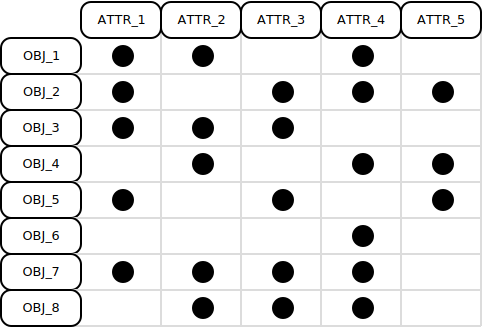
\includegraphics[width=\textwidth]{img/cogito/context_matrix}
    \\ Matrix representation
  \end{minipage}
  \hfill
  \begin{minipage}[t]{0.45\textwidth}
    \vspace{0pt}
    \centering
    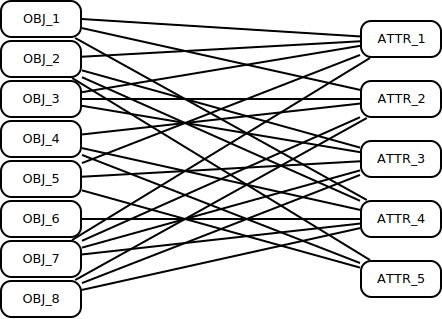
\includegraphics[width=\textwidth]{img/cogito/context_graph}
    \\ Graph representation
  \end{minipage}
\end{figure}
\item \textbf{``Episodic memory"}: list of ``episodes" (lists of objects).
\end{itemize}
\end{block}

\end{frame}

%-------------------------------------------------------------------------------
% BOARD ENCODING
%-------------------------------------------------------------------------------
\subsection{Encoding configurations}

\begin{frame}{``Cogito" system overview}{Encoding configurations}

\begin{block}{First-order logic}

\begin{figure}[ht]
  \begin{minipage}[t]{0.4\linewidth}
    \vspace{0pt}
    \centering
    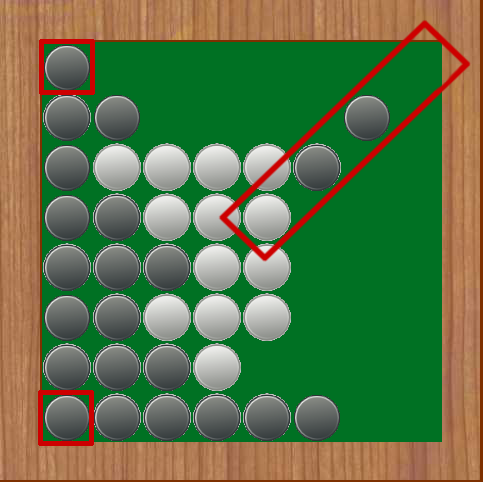
\includegraphics[width=0.8\textwidth]{img/cogito/raisonneur_choix_2}	
  \end{minipage}
  \hfill
  \begin{minipage}[t]{0.55\textwidth}
    \vspace{0pt}
    \begin{itemize}
	\item $isCorner(x) \wedge isMine(x)$
	\item $isMine(w) \wedge isOpp(x) \wedge isOpp(y) 
		  \wedge aligned(w,x,y) \wedge isEmpty(z) 
		  \wedge aligned (x,y,z)$
    \end{itemize}
  \end{minipage}
\end{figure}


  \begin{itemize}
    \item translation- and rotation-invariant,
    \item pattern-matching using homomorphisms.
  \end{itemize}
\end{block}



\end{frame}

%-------------------------------------------------------------------------------
% EVALUATING CONFIGURATIONS
% When the game ends the final configuration is given a value based on whether the 
% agent has won or last. This value and is propagated backwards through previous
% board states with linear attenuation. The value of a state board influences the value 
% of its configurations.
%-------------------------------------------------------------------------------
\subsection{Evaluating configurations}
\begin{frame}{``Cogito" system overview}{Evaluating configurations}

\begin{block}{When the game ends\ldots}
\begin{enumerate}
\item Fixed utilities for win/loss/stalemate configurations,
\item value is propagated back through episode,
\item configuration utility values are adjusted.
\end{enumerate}
\end{block}


\end{frame}

%-------------------------------------------------------------------------------
% GENERATING NEW CONFIGURATIONS
%-------------------------------------------------------------------------------
\subsection{Generating configurations}
\begin{frame}{``Cogito" system overview}{Generating configurations}

\begin{itemize}
\item Start with a configuration shared by two winning/losing board-states,
\item<2> attempt to extend the configuration locally.
\end{itemize}

\begin{figure}[ht]
  \begin{minipage}[t]{0.4\linewidth}
    \vspace{0pt}
    \centering
    \includegraphics<1-1>[width=\textwidth]{img/cogito/build_a1}	
    \includegraphics<2-2>[width=\textwidth]{img/cogito/build_a2}	
  \end{minipage}
  \hfill
  \begin{minipage}[t]{0.4\linewidth}
    \vspace{0pt}
    \centering
    \includegraphics<1-1>[width=\textwidth]{img/cogito/build_b1}
    \includegraphics<2-2>[width=\textwidth]{img/cogito/build_b2}		
  \end{minipage}
\end{figure}

\end{frame}

%-------------------------------------------------------------------------------
% PUTTING IT ALL TOGETHER
%-------------------------------------------------------------------------------
\subsection{Putting it all together}
\begin{frame}{``Cogito" system overview}{Putting it all together}

\begin{block}{It's as easy as\dots}
\begin{enumerate}
\item \textbf{Receive} a set of legal moves,
\item \textbf{evaluate} each resulting state,
\item \textbf{pick} the move resulting in the ``best" state.
\end{enumerate}  
\end{block}

\begin{block}{Possible extensions}
\begin{itemize}
\item Combine with \textbf{MiniMax} for look-ahead,
\item what about \textbf{FCA}?
\end{itemize}
\end{block}

\end{frame}